% subtempl.tex
% -------------------------------------------

Policy-based design \cite{Alexandrescu:2001:MCD} assembles a class
(called \emph{host}) with complex behavior out of many small behaviors
(called \emph{policies}). Each policy defines an interface for a
specific behavior. Following this design principle, we implement a
generic subdivision solution as a \emph{refinement function\/}
parameterized with the \emph{stencils}. The host, i.e., the refinement
function, conducts the \tr\ and applies the stencils provided by the
policies for the \gm s. We provide different hosts and different
policies that can be combined to form subdivision schemes.

We demonstrate the principle with the Catmull-Clark 
subdivision and the Doo-Sabin subdivision. 
A Catmull-Clark subdivision function is structured 
as a primal quadralization function parameterized 
with the policies of the Catmull-Clark stencils.
\begin{lstlisting}
void CatmullClark_subdivision(Polyhedron& p) {
  quadralize_polyhedron<CatmullClark_rule<Polyhedron>>(p);
}
class CatmullClark_rule {
public:
  void facet_rule(  Facet_handle  facet, Point& pt);
  void edge_rule(Halfedge_handle   edge, Point& pt);
  void vertex_rule(Vertex_handle vertex, Point& pt);
};
\end{lstlisting}
The \CodeFmt{quadralize\_polyhedron<>()} is the host function
refining the input mesh
and the \CodeFmt{CatmullClark\_rule} is the policy class applying the
Catmull-Clark stencils. The \CodeFmt{quadralize\_polyhedron<>()} 
refines the control mesh while maintaining the 
correspondence with the stencil, i.e., the submesh centered 
around the given facet, edge, or
vertex, and the smoothing point. The smoothing point
is calculated by calling the policies, i.e.,
the \CodeFmt{facet\_rule()}, the \CodeFmt{edge\_rule()},
and the \CodeFmt{vertex\_rule()} respectively.
%Different refinement scheme may require a 
%different set of stencils. A PQQ scheme needs the
%facet-, edge- and vertex-stencils whereas a DQQ scheme 
%only needs the corner-stencils (Fig.\ref{fig:RefMap}).

\noindent\textbf{Geometry Policies}.
Inside a policy, applying the stencil is simplified to
the mesh traversal of a 1-ring neighborhood. We can use circulators
again, as in the following example for the policy of the facet-stencil 
in the Catmull-Clark subdivision.
\begin{lstlisting}
void CatmullClark_rule::facet_rule(Facet_handle facet, Point& pt) {
  Halfedge_around_facet_circulator hcir = facet->facet_begin();
  Vector vec = hcir->vertex()->point() - ORIGIN;
  ++hcir;
  do {
    vec = vec + hcir->vertex()->point();
  } while (++hcir != facet->facet_begin());
  pt = ORIGIN + vec/circulator_size(hcir);
}
\end{lstlisting}
The \CodeFmt{Facet\_handle facet} points to the 
center facet of the stencil and the \CodeFmt{Point\& pt} 
specifies the smoothing point. We compute the centroid with a
circulator loop over the halfedges surrounding a facet. The \cgal\
geometric kernel is used with point and vector arithmetic.
However, for a specialized kernel, special computations may be 
done in user-defined policies.
 
\noindent\textbf{The refinement host based on Euler operations}.
Implementing the topology refinement is a complex task. One
approach is to encode the refinement into \emph{a sequence of Euler
operations}. For Catmull-Clark subdivision, the refinement is encoded
as edge-vertex insertions, an edge insertion between two neighboring
edge-vertices, a facet-vertex insertion on the inserted edge, and 
edge insertions between the facet-vertex and the edge-vertices 
(Fig~.\ref{fig:CCRefinement}). These are Euler operations supported 
by \cgalpoly.
\begin{figure}
  \centering
  \epsfig{file=figs/CCRefinement.eps, width=7cm}
  \caption{A PQQ refinement of a facet is encoded into a sequence of
  vertex insertions and edge insertions. Red indicates the inserted
  vertices and edges in each step.}
  \label{fig:CCRefinement}
\end{figure}

The correspondence between stencil and control mesh is assured in the
refinement with a consistent \emph{traversal sequence\/} on the mesh.
The refinement host has a two pass algorithm, hence two traversals.
The first pass generates the points by calling the policies. The
second pass refines the mesh with a sequence of the Euler operations.
The points generated in the first pass are stored in a point buffer in
the order of the stencil traversal. The sequence of the vertex
insertions is consistent to match the stencil traversal, i.e.\ the
storage order of the point buffer.
% It assures the stencil correspondence of the refinement.

\noindent\textbf{The refinement host based on the modifier callback mechanism}.
Most primal refinement schemes can be translated into a sequence of
Euler operations. Though dual schemes, e.g.\ Doo-Sabin subdivision,
have no simple translation of Euler operations. A sequence of Euler
operations for a DQQ scheme consist of two times of the midedge
refinement \cite{Peters:1997:SSS} and result an inefficient
implementation. This multipass refinement scheme, called subdivision
operator factorization, is introduced in \cite{Peter:2003:CPDSS}.  To
support such schemes efficiently, we use the modifier callback
mechanism and the incremental builder of \cgalpoly\ to rebuild the
mesh connectivity. In addition to the point buffer, we also create a
facet list based on the source mesh. Note that in a DQQ scheme, every
new facet corresponds to a vertex, edge or facet. The combination of
the points buffer and facet list represent a facet-vertex index list
which indexes the vertices and enumerates each facet as an index
sequence. A modifier creating a polyhedron from a facet-vertex index
list is then a simple task, here the sketch using the incremental
builder \CodeFmt{pb}.
\begin{lstlisting}
pb.begin_surface(num_point, num_facet); {
  for (int i = 0; i < num_point; ++i) 
    pb.add_vertex(Point(point_buffer[i*3+0], 
                        point_buffer[i*3+1], 
                        point_buffer[i*3+2]));        
  for (int i = 0; i < num_facet; ++i) {
    pb.begin_facet();
    for (int n = 0; n < facet_buffer[i][0]; ++n)
      pb.add_vertex_to_facet(facet_buffer[i][n+1]);
    pb.end_facet();
  }
}
pb.end_surface();
\end{lstlisting}

\begin{figure}
  \centering
  \epsfig{file=figs/plane0.eps, width=2.35cm} \\
  \epsfig{file=figs/planeCC1.eps, width=2.35cm}
  \epsfig{file=figs/planeCC2.eps, width=2.35cm}
  \epsfig{file=figs/planeCC.eps, width=2.35cm}\\
  \epsfig{file=figs/planeDS1.eps, width=2.35cm}
  \epsfig{file=figs/planeDS2.eps, width=2.35cm}
  \epsfig{file=figs/planeDS.eps, width=2.35cm}
  \caption{Catmull-Clark subdivision surfaces ({\itshape second row}) and
  Doo-Sabin subdivision surfaces ({\itshape third row}) 
  of an aircraft polyhedron ({\itshape first row}).
  }
  \label{fig:SubExample}
\end{figure}

\noindent\textbf{The subdivision library.}
Our subdivision design solution, decoupling the geometry rules from
the refinement, grants users flexible control of the stencils.
Variants of subdivisions can be devised by simply combining different
refinement hosts and geometric policies.  A combinatory subdivision
set is provided within our subdivision library. It includes
Catmull-Clark subdivision, Doo-Sabin subdivision, Loop subdivision,
Quad-Triangle subdivision and $\sqrt{3}$ subdivision. Since \cgalpoly\ 
supports non-uniform meshes (in contrast to the quad-tree or
patch-based implementation), chains of different refinements are
naturally supported.
%\begin{lstlisting}
%void MySubdivision(Polyhedron& p) {
%  quadralize_polyhedron<Myrule_1<Polyhedron>>(p);
%  dualize_polyhedron<Myrule_2<Polyhedron>>(p);
%} 
%\end{lstlisting}
Furthermore, our solution is parameterized with the mesh structure and
can thus be applied to user-specialized versions of \cgalpoly.  Note
that no special flag or attribute is required to assist the \tr . This
generality makes our solution naturally fit in a modeling pipeline or a
multipass modeling environment.
%In some applications, efficiency is more
%important than flexibility. An efficient implementation
%of $\sqrt{3}$ based on \cgalpoly\ is introduced in next 
%section.

%TODO: since the writing memory is not overlapped, multi-threaded
%supporting is easily done.

%TODO: trade-off between generic and efficient.
 
